\documentclass[tikz,border=6pt]{standalone}
\usepackage{xcolor}

\definecolor{blockblue}{HTML}{4A90D9}

\begin{document}
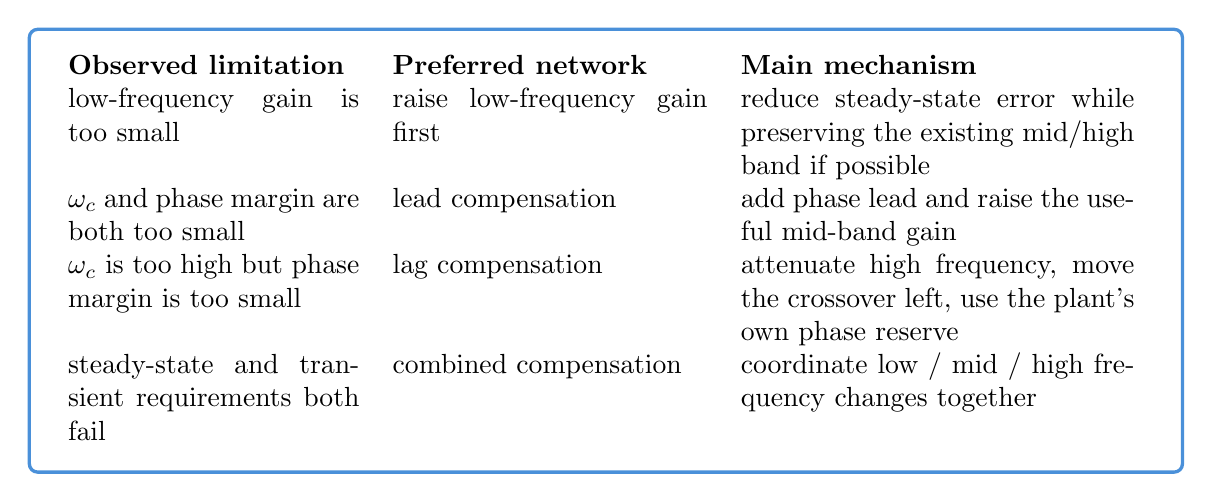
\begin{tikzpicture}[line width=1.2pt]
  \node[
    draw=blockblue,
    rounded corners=3pt,
    inner sep=8pt,
    align=left
  ] at (0,0) {
    \begin{tabular}{p{3.7cm}p{4.0cm}p{5.0cm}}
      \textbf{Observed limitation} & \textbf{Preferred network} & \textbf{Main mechanism} \\
      low-frequency gain is too small & raise low-frequency gain first & reduce steady-state error while preserving the existing mid/high band if possible \\
      $\omega_c$ and phase margin are both too small & lead compensation & add phase lead and raise the useful mid-band gain \\
      $\omega_c$ is too high but phase margin is too small & lag compensation & attenuate high frequency, move the crossover left, use the plant's own phase reserve \\
      steady-state and transient requirements both fail & combined compensation & coordinate low / mid / high frequency changes together \\
    \end{tabular}
  };
\end{tikzpicture}
\end{document}
